\documentclass{beamer}
\usepackage[utf8]{inputenc}  % 输入字符集为UTF-8
\usepackage{ctex}  % 支持中文
\usepackage{amsmath}  % 支持数学符号
\usepackage{hyperref}  % 支持超链接
\usepackage{graphicx}  % 插入图片

\usetheme{Antibes}  % 使用 Antibes 主题
\usefonttheme{serif}  % 使用衬线字体主题

\title{动态规划背包模型 + 线性 DP}
\author{ncst acm集训队\\ 林凯}
\date{\today}

\begin{document}

\frame{\titlepage}

\section{什么是dp?}

\begin{frame}{DP(Dynamic programming) 既动态规划问题}
    动态规划是一种将一个复杂问题分解为多个简单的子问题求解的方法。将子问题的答案存储在记忆数据结构中,当子问题再次需要解决时,只需查表查看结果,而不需要再次重复计算,因此节约了计算时间。
\end{frame}

\section{动态规划基本概念}

\begin{frame}{最优子结构}
    最优子结构是动态规划问题的一个重要特征。它意味着一个最优解可以由其子问题的最优解构成。换句话说,如果我们能够找到子问题的最优解,那么就可以通过组合这些子问题的解来构建原问题的最优解。
\end{frame}

\begin{frame}{重叠子问题}
    重叠子问题指的是在求解一个问题的过程中,需要多次求解一些相同的子问题。如果我们能够将这些子问题的解存储起来,就可以避免重复计算,从而提高效率。
\end{frame}

\begin{frame}{状态转移方程}
    状态转移方程是动态规划的核心,它描述了当前状态与之前状态之间的关系。通过状态转移方程,我们可以将一个复杂的问题分解为更简单的子问题,并利用子问题的解来构建原问题的解。
\end{frame}

\begin{frame}{记忆化搜索}
    记忆化搜索是动态规划的一种实现方式。它通过维护一个存储结构(如哈希表或数组)来记录已经计算过的子问题的解,从而避免重复计算。当需要求解一个子问题时,首先检查它是否已经被计算过,如果是,直接返回存储的结果;否则,计算该子问题的解并将其存储起来。
\end{frame}

\section{常见dp问题}

\begin{frame}{线性 DP}
    线性 DP 是动态规划中最基本的一类问题,通常可以通过递推或迭代的方式解决。常见的例子有斐波那契数列和最长上升子序列问题。
\end{frame}

\begin{frame}{区间 DP}
    区间 DP 适用于将问题划分为若干个连续子区间来求解的情况。通过合并子区间的解,可以得到整个问题的最优解。典型应用包括矩阵连乘问题和石子合并问题。
\end{frame}

\begin{frame}{背包 DP}
    背包 DP 主要用于解决选择问题,即在给定约束条件下,如何选择物品以使得总价值最大。常见的背包问题包括01背包、完全背包和多重背包。
\end{frame}

\begin{frame}{树形 DP}
    树形 DP 主要用于树结构上的动态规划问题。利用树的递归结构,按照后序遍历的顺序求解。常见应用有二叉树的最大路径和问题。
\end{frame}

\begin{frame}{状态压缩 DP}
    状态压缩 DP 适用于问题的状态空间较大但具有特定规律的情况。通过压缩状态表示,可以显著降低时间和空间复杂度。典型应用包括旅行商问题。
\end{frame}

\begin{frame}{数位 DP}
    数位 DP 用于处理与数字相关的问题,尤其是涉及到数字特定位数的约束问题。通过按位动态规划,可以高效地解决这类问题,如计数满足特定条件的数字个数。
\end{frame}

\begin{frame}{计数型 DP}
    计数型 DP 主要用于统计满足某些条件的解的个数。例如,计算某个序列中满足特定条件的子序列数量。
\end{frame}

\begin{frame}{递推型 DP}
    递推型 DP 是通过定义递推关系来求解问题的类型。通过逐步计算更大的子问题的解,最终得到原问题的解。
\end{frame}

\begin{frame}{概率型 DP}
    概率型 DP 适用于需要计算某些事件发生概率的问题。常用于博弈问题或随机过程的期望计算。
\end{frame}

\begin{frame}{博弈型 DP}
    博弈型 DP 主要用于分析双人对抗类问题的最优策略。通过考虑不同玩家的策略,可以得出每一步的最优解。
\end{frame}

\begin{frame}{记忆化搜索}
    记忆化搜索是将动态规划的递归实现进行优化的一种方法。通过在递归过程中存储已经计算过的结果,避免重复计算,从而提高效率。
\end{frame}

\section{线性dp基础}

\begin{frame}{斐波那契数列 (洛谷B2064)}
    斐波那契数列是指这样的数列:数列的第一个和第二个数都为 $1$,接下来每个数都等于前面 $2$ 个数之和。给出一个正整数 $a$,要求斐波那契数列中第 $a$ 个数是多少。
\end{frame}

\begin{frame}{解题思路}
    这道题可以使用动态规划来解决。我们定义一个数组 $f$,其中 $f[i]$ 表示第 $i$ 个斐波那契数。初始时,我们设定 $f[1] = 1$,$f[2] = 1$。然后通过递推关系式 $f[i] = f[i-1] + f[i-2]$ 计算出第 $a$ 个斐波那契数。
\end{frame}

\begin{frame}{最长上升子序列(洛谷B3637)}
    给出一个由 $n(n\le 5000)$ 个不超过 $10^6$ 的正整数组成的序列。请输出这个序列的\textbf{最长上升子序列}的长度。最长上升子序列是指,从原序列中\textbf{按顺序}取出一些数字排在一起,这些数字是\textbf{逐渐增大}的。
\end{frame}

\begin{frame}{解题思路}
    我们可以使用动态规划来解决这个问题。定义一个数组 $f$,其中 $f[i]$ 表示以第 $i$ 个元素结尾的最长上升子序列的长度。初始时,$f[i] = 1$,表示每个元素自身构成一个序列。对于每个 $i$,我们检查所有之前的元素 $j$,如果 $a[j] < a[i]$,则更新 $f[i] = \max(f[i], f[j] + 1)$。最终答案是 $f$ 数组中的最大值。
\end{frame}

\begin{frame}{数字三角形(洛谷P1216)}
    观察下面的数字金字塔。写一个程序来查找从最高点到底部任意处结束的路径,使路径经过数字的和最大。每一步可以走到左下方的点也可以到达右下方的点。
    \begin{figure}
        \centering
        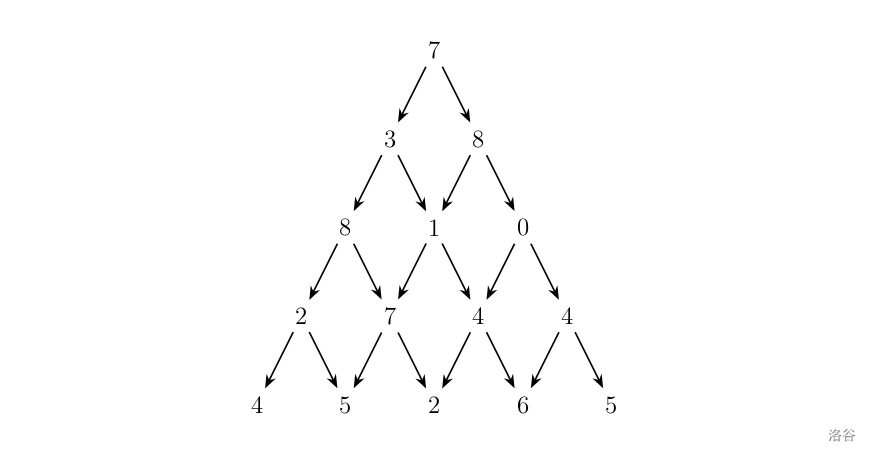
\includegraphics[width=0.5\textwidth]{./ex.png}
    \end{figure}
    在上面的样例中,从 $7 \rightarrow 3 \rightarrow 8 \rightarrow 7 \rightarrow 5$ 的路径产生了最大权值。
\end{frame}

\begin{frame}{解题思路}
    我们可以使用自底向上的动态规划来解决这个问题。定义 $f[i][j]$ 表示从点 $(i, j)$ 到底部任意点的最大路径和。初始时,我们将底部的元素值赋给 $f$,然后递推计算出上层元素的最大路径和。最终 $f[1][1]$ 就是所求的最大路径和。
\end{frame}

\begin{frame}{最长公共子序列(洛谷P1439)}
    给出 $1, 2, \dots, n$ 的两个排列 $P_1, P_2$,请问 $P_1$ 和 $P_2$ 的\textbf{最长公共子序列}有多长?其中,$1\leq n\leq 3000$。
\end{frame}

\begin{frame}{解题思路}
    可以使用动态规划解决。定义一个二维数组 $f$,其中 $f[i][j]$ 表示 $P_1$ 的前 $i$ 个元素和 $P_2$ 的前 $j$ 个元素的最长公共子序列长度。递推关系为 $f[i][j] = \max(f[i-1][j], f[i][j-1])$,如果 $P_1[i] == P_2[j]$,则 $f[i][j] = f[i-1][j-1] + 1$。最终 $f[n][n]$ 即为所求。
\end{frame}

\begin{frame}{编辑距离 (P2758)}
    设 $A$ 和 $B$ 是两个字符串。我们要用最少的字符操作次数,将字符串 $A$ 转换为字符串 $B$。这里所说的字符操作共有三种:
    \begin{itemize}
        \item 删除一个字符;
        \item 插入一个字符;
        \item 将一个字符改为另一个字符。
    \end{itemize}
    $A, B$ 均只包含小写字母。
\end{frame}

\begin{frame}{解题思路}
    定义一个二维数组 $f$,其中 $f[i][j]$ 表示将 $A$ 的前 $i$ 个字符转换为 $B$ 的前 $j$ 个字符所需的最少操作次数。递推关系为 $f[i][j] = \min(f[i-1][j] + 1, f[i][j-1] + 1, f[i-1][j-1] + cost)$,其中 $cost = 0$ 如果 $A[i] = B[j]$,否则 $cost = 1$。最终 $f[m][n]$ 即为所求的编辑距离。
\end{frame}

\section{背包问题}

\begin{frame}{01背包}
    有n件物品和一个最多能背重量为w 的背包。第i件物品的重量是$weight[i]$,得到的价值是$value[i]$。每件物品只能用一次,求解将哪些物品装入背包里物品价值总和最大。
\end{frame}

\begin{frame}{解题思路}
    定义一个数组 $f$,其中 $f[j]$ 表示背包容量为 $j$ 时的最大价值。初始时,$f[0] = 0$。然后对于每件物品 $i$,倒序更新 $f[j] = \max(f[j], f[j - weight[i]] + value[i])$。最终 $f[w]$ 就是背包能装下的最大价值。
\end{frame}

\begin{frame}{贪心选择策略不适用于0-1背包问题}
    对于0-1背包问题,贪心选择之所以不能得到最优解是因为,在这种情况下,它无法保证最终能将背包装满,部分闲置的背包空间使每千克背包空间的价值降低了。 事实上,在考虑0-1背包问题时,应比较选择该物品和不选择该物品所导致的最终方案,在做出最好选择。由此可导出许多互相重叠的子问题。这正是该问题可用动态规划算法求解的另一重要特征。
\end{frame}

\begin{frame}{完全背包}
    有N件物品和一个最多能背重量为W的背包。第i件物品的重量是$weight[i]$,得到的价值是$value[i]$。每件物品都有无限个(也就是可以放入背包多次),求解将哪些物品装入背包里物品价值总和最大。
\end{frame}

\begin{frame}{解题思路}
    和01背包问题类似,区别在于更新状态时,需要正序更新。定义数组 $f[j]$ 表示背包容量为 $j$ 时的最大价值。对于每件物品 $i$,正序更新 $f[j] = \max(f[j], f[j - weight[i]] + value[i])$。
\end{frame}

\begin{frame}{多重背包}
    有N件物品和一个最多能背重量为W的背包。第i件物品的重量是$weight[i]$,得到的价值是$value[i]$。对于每件物品i都有$a[i]$个(也就是可以放入背包a[i]次),求解将哪些物品装入背包里物品价值总和最大。
\end{frame}

\begin{frame}{解题思路}
    我们可以将多重背包问题转化为01背包问题。具体来说,对于每件物品 $i$,将其分解成若干个物品,每个物品的重量和价值保持不变,然后利用01背包的算法求解。或者,我们可以使用二进制优化的方法,将 $a[i]$ 分解为若干个物品,使得原问题中的多重约束转化为多个01背包问题。
\end{frame}

\begin{frame}{分组背包}
    有n件物品和一个最多能背重量为w 的背包。将n件物品分为m组,每组物品有若干个,同一组内的物品最多只能选一个。第i件物品的重量是$weight[i]$,得到的价值是$value[i]$。每件物品只能用一次,求解将哪些物品装入背包里物品价值总和最大。
\end{frame}

\begin{frame}{解题思路}
    定义数组 $f[j]$ 表示背包容量为 $j$ 时的最大价值。对于每一组物品,选择其中一个物品更新 $f$ 数组。具体做法是,对于每组中的每一个物品,更新 $f[j] = \max(f[j], f[j - weight[i]] + value[i])$。
\end{frame}

\begin{frame}{}
    \centering
    \Huge the end
\end{frame}

\end{document}
